\documentclass[twocolumn, prl, superscriptaddress]{revtex4}
%\documentclass[reprint, prl, aps, showpacs]{revtex4-1}
%\documentclass[preprint, aps, showpacs]{revtex4-1}

\usepackage{graphicx}
\usepackage{amsmath,amssymb}
%\usepackage[usenames,dvipsnames]{color}
%\usepackage[colorlinks=true, citecolor=blue, linkcolor=WildStrawberry]{hyperref}
%\usepackage[citecolor=blue]{hyperref}
%\usepackage[justification=centerfirst]{caption}
\usepackage{epstopdf}

%\usepackage[latin1]{inputenc}
\usepackage{tikz}
\usetikzlibrary{shapes,arrows}

\newcommand{\braket}[2]{\left\langle#1\, |\,#2\,\right\rangle}  %  < #1 | #2 >
\newcommand{\expec}[1]{\langle#1\rangle}  %  < #1 >
\newcommand{\drm}{{\rm d}}
\newcommand{\irm}{{\rm i}}
\newcommand{\beq}{\begin{equation}}
\newcommand{\eeq}{\end{equation}}
\newcommand{\bdm}{\begin{displaymath}}
\newcommand{\edm}{\end{displaymath}}
\newcommand{\T}[1]{\tilde{#1}}
\newcommand{\wT}[1]{\widetilde{#1}}
\newcommand{\Cdot}{\!\cdot\!}
\newcommand{\SNR}{\textnormal{SNR}}
\newcommand{\rednote}[1]{{\color{red} (#1)}}
\newcommand{\fixme}[1]{\textcolor{green}{\textbf{\textit{{#1}}}}}

\DeclareFontFamily{OT1}{pzc}{}
\DeclareFontShape{OT1}{pzc}{m}{it}{<-> s * [1.10] pzcmi7t}{}
\DeclareMathAlphabet{\mathpzc}{OT1}{pzc}{m}{it}

\def\dblone{\hbox{$1\hskip -1.2pt\vrule depth 0pt height 1.6ex width 0.7pt \vrule depth 0pt height 0.3pt width 0.12em$}}

\graphicspath{{./plots/}}
\begin{document}

\title{Limiting the effects of earthquakes on gravitational-wave interferometers}

\author{Michael Coughlin}
\affiliation{Department of Physics, Harvard University, Cambridge, MA 02138, USA}

\author{Paul Earle}
\affiliation{United States Geological Survey, Golden, CO 80401, USA}

\author{Jan Harms}
\affiliation{INFN, Sezione di Firenze, Sesto Fiorentino, 50019, Italy\\
Universit\`a degli Studi di Urbino ``Carlo Bo'', I-61029 Urbino, Italy}

\author{Sebastien Biscans}
\affiliation{LIGO Laboratory, Massachusetts Institute of Technology, Cambridge, MA 02138, USA}

\author{Christopher Buchanan}
\affiliation{Department of Physics and Astronomy, Louisiana State University, Baton Rouge, LA 70803-4001, USA}

\author{Eric Coughlin}
\affiliation{Department of Computer Science, Luther College, 700 College Dr, Decorah, IA 52101, USA}

\author{Fred Donovan}
\affiliation{LIGO Laboratory, Massachusetts Institute of Technology, Cambridge, MA 02138, USA}

\author{Jeremy Fee}
\affiliation{United States Geological Survey, Golden, CO 80401, USA}

\author{Hunter Gabbard}
\affiliation{Albert-Einstein-Institut, Max-Planck-Institut f{\"u}r Gravitationsphysik, D-30167 Hannover, Germany}

\author{Michelle Guy}
\affiliation{United States Geological Survey, Golden, CO 80401, USA}

\author{Nikhil Mukund}
\affiliation{Inter-University Centre for Astronomy and Astrophysics, Ganeshkhind, Pune University Campus Pune 411 007, India}

\author{Matthew Perry}
\affiliation{Planetary Science Institute, Lakewood, CO 80401, USA}


\begin{abstract}

Ground-based gravitational wave interferometers such as the Laser Interferometer Gravitational-wave Observatory (LIGO) are susceptible to high-magnitude teleseismic events, which can interrupt their operation in science mode and significantly reduce the duty cycle. It can take several hours for a detector to stabilize enough to return to its nominal state for scientific observations. The down time can be reduced if advance warning of impending shaking is received and the impact is suppressed in the isolation system with the goal of maintaining stable operation even at the expense of increased instrumental noise. Here we describe an early warning system for modern gravitational-wave observatories. The system relies on near real-time earthquake alerts provided by the U.S. Geological Survey (USGS) and the National Oceanic and Atmospheric Administration (NOAA).  Hypocenter and magnitude information is generally available in 5 to 20 minutes of a significant earthquake depending on its magnitude and location.  The alerts are used to estimate arrival times and ground velocities at the gravitational-wave detectors.  In general, 90\% of the predictions for ground-motion amplitude are within a factor of 5 of measured values.  The error in both arrival time and ground-motion prediction introduced by using preliminary, rather than final, hypocenter and magnitude information is minimal. By using a machine learning algorithm, we develop a prediction model that calculates the probability that a given earthquake will prevent a detector from taking data.   Our initial results indicate that by using detector control configuration changes, we could prevent interruption of operation from 40-100 earthquake events in a 6-month time-period.

\end{abstract}

\maketitle

\section{Introduction}
\label{sec:Intro}

Earthquakes are a significant issue for gravitational-wave detectors. In previous work \cite{CoSt2015}, it is described how large-scale astronomical experiments, such as meter class telescopes and gravitational-wave interferometers, are susceptible to earthquakes. In the case of telescopes, the predominant concern is the potential for nearby, devastating earthquakes, which will damage either the surrounding structure or the mirrors that make up the telescope, and it is argued that a regional early earthquake warning (EEW) \cite{Al2012,KuAl2013a,KuAl2013b,KuHe2014,CoLa2009a,CoLa2009b,BoAl2014,HoKa2008,HoEA2011c,StAl2016} system is important to minimize potential damage to telescopes. 
Gravitational-wave detectors, on the other hand, are susceptible to teleseismic events from around the world \cite{MaFa2012}. 
The two detectors of the Laser Interferometer Gravitational-wave Observatory (LIGO) \cite{aligo} that have made the first direct observations of gravitational waves \cite{AbEA2016a,AbEA2016e} form a global network of gravitational-wave interferometers together with the Virgo \cite{avirgo}, and GEO600 \cite{Gr2010} detectors. These detectors can be destabilized by significant ground motion, despite seismic isolation systems designed to minimize such effects \cite{AbAd2002,StAb2009,MaLa2015}.

During the last LIGO science run, large amplitude earthquakes from around the world would typically cause the detectors to fall out of lock \cite{CoSt2015}, which signifies a failure of the control system to maintain optics at their nominal positions and orientations with subsequent loss of laser power in the system. Not only were the data around the time of the earthquakes not useful for gravitational-wave detection, but it would also take hours of dead time for the detectors to return to the locked state. 
We showed that there are potential gains to be made with an early warning system assuming that the incurred downtime could be reduced with sufficient advance notice of the earthquakes' arrivals.
Detailed studies of earthquake response during previous science runs showed that there is about one teleseismic event each week producing ground motion at the sites too strong for the control system to be able to maintain lock. In most cases, it was then impossible to lock the interferometer for some hours. A scheme that would suppress disturbances of earthquakes early in the isolation system with the final goal to maintain lock during strong ground motion, even at the price of increased instrumental noise, could potentially lead to substantial increase of the duty cycle. This will likely be of greater importance even in high-power configurations of the advanced detectors, where thermalization of test masses during the locking procedure could potentially increase the time it takes to reach maximal sensitivity.

For this reason, we have created an earthquake early warning client named \emph{Seismon}, which uses a real-time event messaging system of the US Geological Survey to mitigate the effects of teleseismic events on ground-based gravitational-wave detectors. The messages contain information about the fault rupture such as location, depth, magnitude. They are received and processed in real time to estimate arrival times of the various seismic phases, and seismic amplitudes of the Rayleigh phase at the detector sites.
In section~\ref{sec:algorithm}, we describe the algorithm.
In section~\ref{sec:performance}, we describe the performance of the algorithm on the most recent gravitational-wave detector data.
In section~\ref{sec:conclusions}, we offer concluding remarks and suggest directions for future research.

\section{Algorithm}
\label{sec:algorithm}

Figure~\ref{fig:flowchart} shows the flowchart for the \emph{Seismon} pipeline, developed to mitigate the effects of teleseismic events on ground-based interferometric gravitational wave detectors. It uses event notices received from USGS and makes time of arrival and amplitude predictions for earthquake seismic phases at sites of current detectors. Using a combination of earthquake magnitude, distance, and depth information, a prediction of the likelihood of the earthquake causing data disruption at the sites is made.

% Define block styles
\tikzstyle{decision} = [diamond, draw, fill=blue!20,
    text width=4.5em, text badly centered, node distance=3cm, inner sep=0pt]
\tikzstyle{block} = [rectangle, draw, fill=blue!20,
    text width=5em, text centered, rounded corners, minimum height=3em]
\tikzstyle{line} = [draw, -latex']
\tikzstyle{cloud} = [draw, ellipse,fill=red!20, node distance=3cm,
    minimum height=2em]
\tikzstyle{emptyblock} = [rectangle, minimum height=3em]

\begin{figure}[t]
 \begin{center}
 \begin{tikzpicture}[node distance = 2.3cm, auto]
    % Place nodes
    \node [emptyblock] (init) {};
    \node [block, left of=init] (PDL) {PDL};
    \node [block, right of=init] (GeoJSON) {GeoJSON};
    \node [block, below of=init] (Parse) {Parse events};
    \node [block, below of=Parse] (Traveltimes) {Calculate travel times};
    \node [block, below of=Traveltimes] (XML) {Produce XML files};
    \node [block, below of=PDL, node distance=9cm] (Plot) {Summary / Plot};
    \node [block, below of=GeoJSON, node distance=9cm] (Epics) {Site Notification};
    % Draw edges
    \path [line] (PDL) -- (Parse);
    \path [line] (GeoJSON) -- (Parse);
    \path [line] (Parse) -- (Traveltimes);
    \path [line] (Traveltimes) -- (XML);
    \path [line] (XML) -- (Plot);
    \path [line] (XML) -- (Epics);
 \end{tikzpicture}
 \end{center}
 \caption{A flow chart of the \emph{Seismon} pipeline. The USGS's Product Distribution Layer (PDL) and public GeoJSON earthquake files provide information used by \emph{Seismon} to compute estimated site arrival times and Rayleigh wave velocities.}
 \label{fig:flowchart}
\end{figure}

\subsection{Notices}

\emph{Seismon} relies on the most preliminary notices of earthquakes currently available generated by worldwide networks of seismometers. In general, the process of identification occurs when a primary or P-wave arrival is identified in a number of nearby seismometers. Preliminary estimates of the location, including latitude, longitude, and depth, are then derived by analyzing ground motion of these first arrivals. Robust earthquake magnitude estimates come later depending on the earthquake magnitude. It is generally challenging to obtain quick estimates of high-magnitude earthquakes, mostly because the fault rupture can last for a minute or more and information thereof resides in slowly evolving surface displacement. Consequently, preliminary estimates often underestimate the magnitude of strong earthquakes as shown in figure \ref{fig:initialfinal}. This data is from all earthquakes from the last science run, comparing the earliest magnitude estimates (as would be used by \emph{Seismon} to the final estimates computed much later).
\begin{figure}[t]
\hspace*{-0.5cm}
\centering
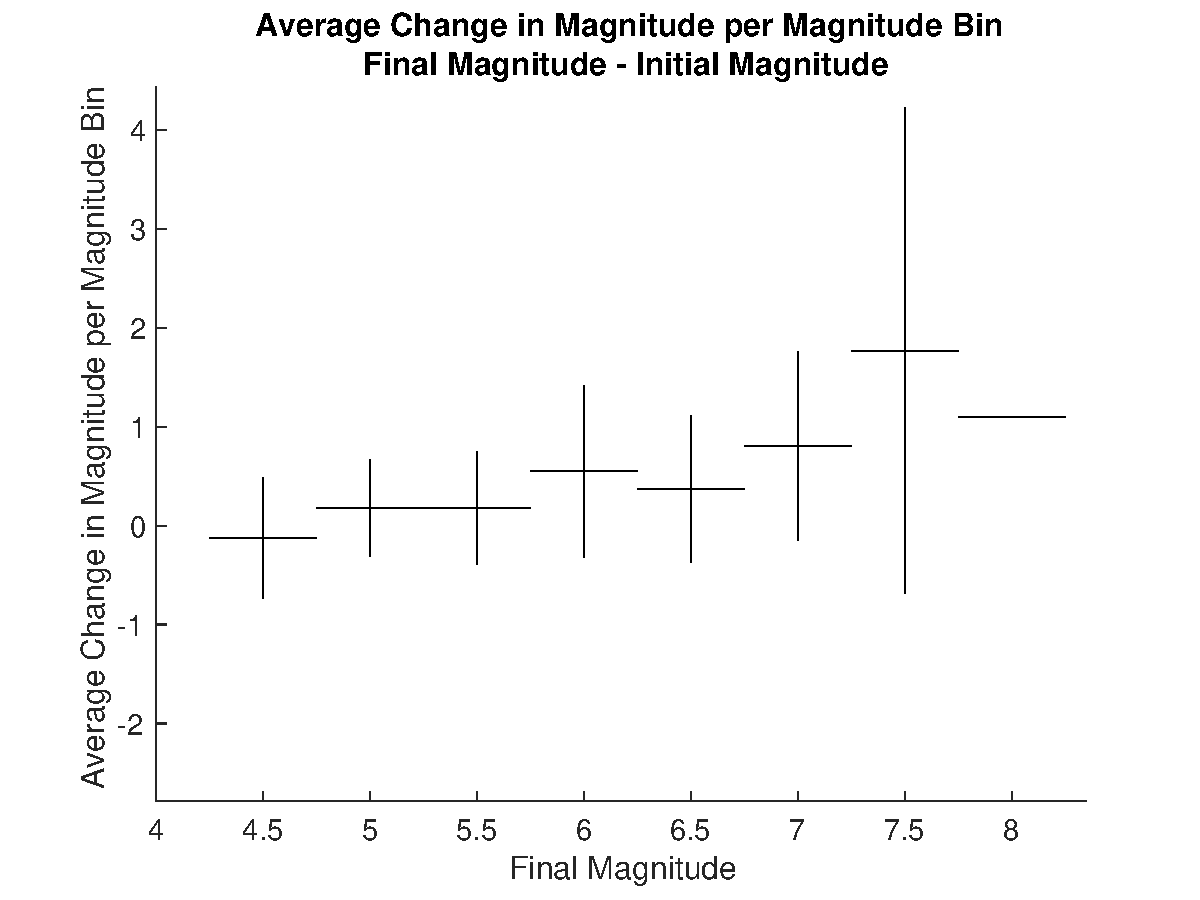
\includegraphics[width=4in]{AverageChange.pdf}
\caption{Comparison of initial versus final magnitude estimates of earthquakes. Magnitudes of strong earthquakes are typically underestimated in preliminary analyses since associated fault ruptures can last up to minutes, and precise information is obtained from slow surface displacements. Estimates of magnitudes for weak earthquakes are less biased in this way when fault ruptures only last for a couple of seconds.}
 \label{fig:initialfinal}
 \end{figure}

For distant epicenters, achievable warning times are mostly determined by the comparison of P-wave travel times relative to secondary or S-waves and surface waves. P-waves travel at about twice the speed of S-waves, and surface waves are delayed further since they are bound to travel along the surface. Surface and S-phases generally have a stronger effect on gravitational-wave detectors due to their higher amplitudes. Furthermore, P-waves produce predominantly vertical motion at the detector sites, S-waves predominantly horizontal motion, while surface Rayleigh waves cause vertical and horizontal ground motion with similar amplitudes. It is likely that these polarization-dependent effects also influence the impact of a seismic phase on the detector.

The United States Geological Survey (USGS) provides a number of channels for information about earthquakes, on different time-scales. The earliest, which we will use in the \emph{Seismon} pipeline, are automated pipelines, which use USGS-supported worldwide networks of seismometers to make earthquake identifications. The earliest solutions provide event source parameters, including both location and magnitude estimates. At later times, moment tensor solutions and finite fault models are calculated from the array data. These solutions are distributed through USGS's Product Distribution Layer (PDL), which has been configured to receive all notifications of earthquakes worldwide. As all USGS-supported networks submit notices through this service, the pipeline is ensured to receive all relevant notices.
In particular, the notification messages are in the form of either EQXML or QuakeML Extensible Markup Language (XML) files, although the distribution also provides image files and other related content depending on the information. Each network that detects an earthquake provides time-tagged versions of their products, which will allow us to estimate the delay induced by the process of earthquake identification and product distribution. This is a cross-platform Java based code that runs constantly on a dedicated machine. 
After these solutions have been vetted, they are also released in public GeoJSON earthquake files available from the USGS website.

\subsection{Analysis}

The second step of the process is to convert event notifications to information about the time of arrival and amplitudes at the sites.
In summary, we use the location and magnitude estimates of the PDL client for two purposes. 
The first is the time of seismic wave arrivals at the gravitational-wave detectors.
The second is the ground motion at the gravitational-wave detectors.
Accurate prediction of the ground velocity amplitude based on earthquake magnitude and distance will be required to limit the false alarms. 
This equation should account for physical effects with variable parameters used to fit to the seismic data currently available.
P- and S-wave arrivals can be accurately determined given latitude, longitude, and depth information by calculating travel times using the iaspei-tau package \cite{Snoke2009} wrapped by Obspy. We can approximate surface waves as having a constant 3.5\,km/s speed value. 

The second step is to make amplitude predictions for each site. We estimate the peak amplitude of the surface waves, $\rm Rf_{amp}$, at the sites using equation (\ref{eq:Rfamp}), which we describe below. This was developed as a fit to historical earthquakes at the gravitational-wave detectors. We chose the peak amplitude as compared to root-mean-squared ground-motion because a root-mean-squared value depends on technical calculation choices, which to be effective will depend on the event in question. Eventually it would be appropriate to determine what observational quantity is best suited to lock loss for the detectors, but for now we adopt peak amplitude due to its relative simplicity. Both the time-of-arrival and amplitude are predicted as a function of distance. This allows users of the algorithm to interpolate these metrics for their locations of interest. In general, we generate the predictions for all currently operating gravitational-wave detectors.

\begin{figure*}[t]
\hspace*{-0.5cm}
 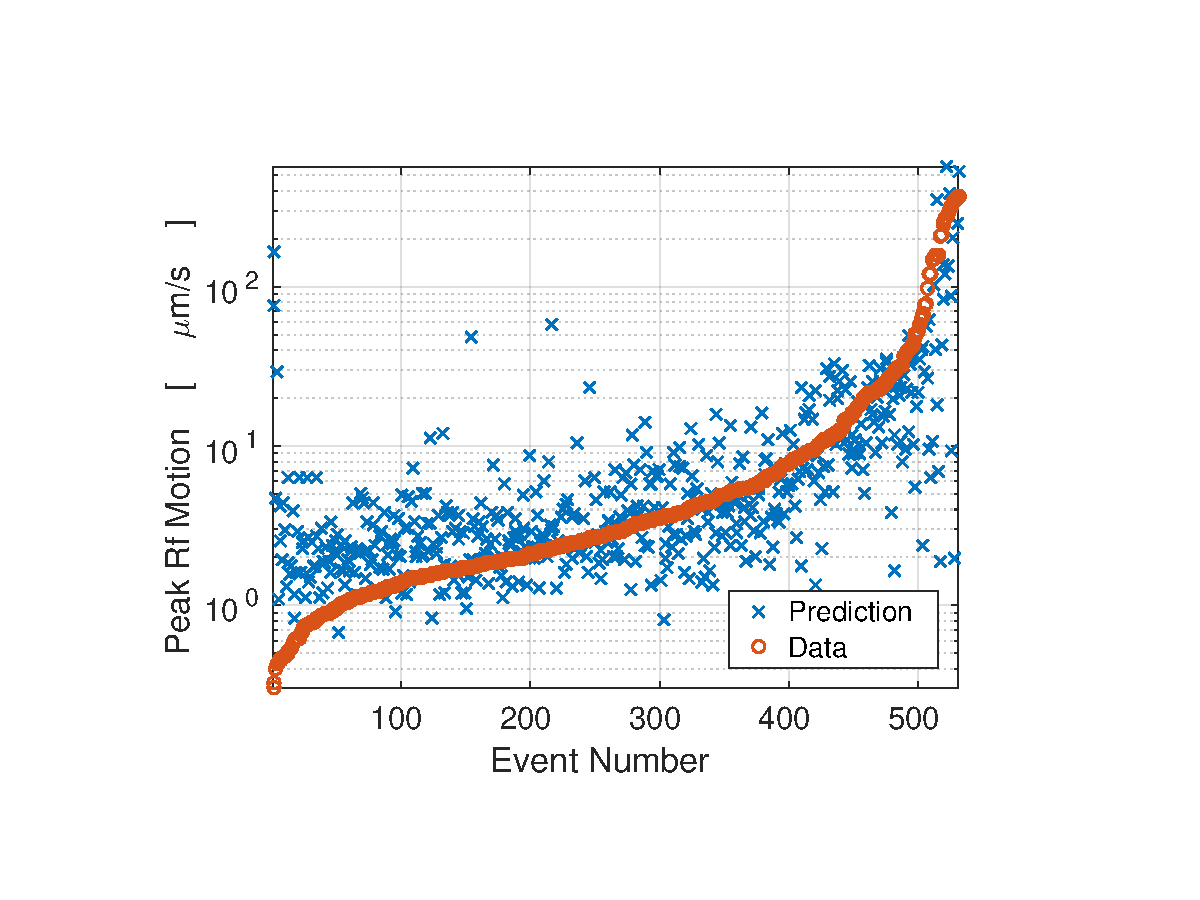
\includegraphics[width=3.5in]{Prediction_LHO_S5_S6.pdf}
 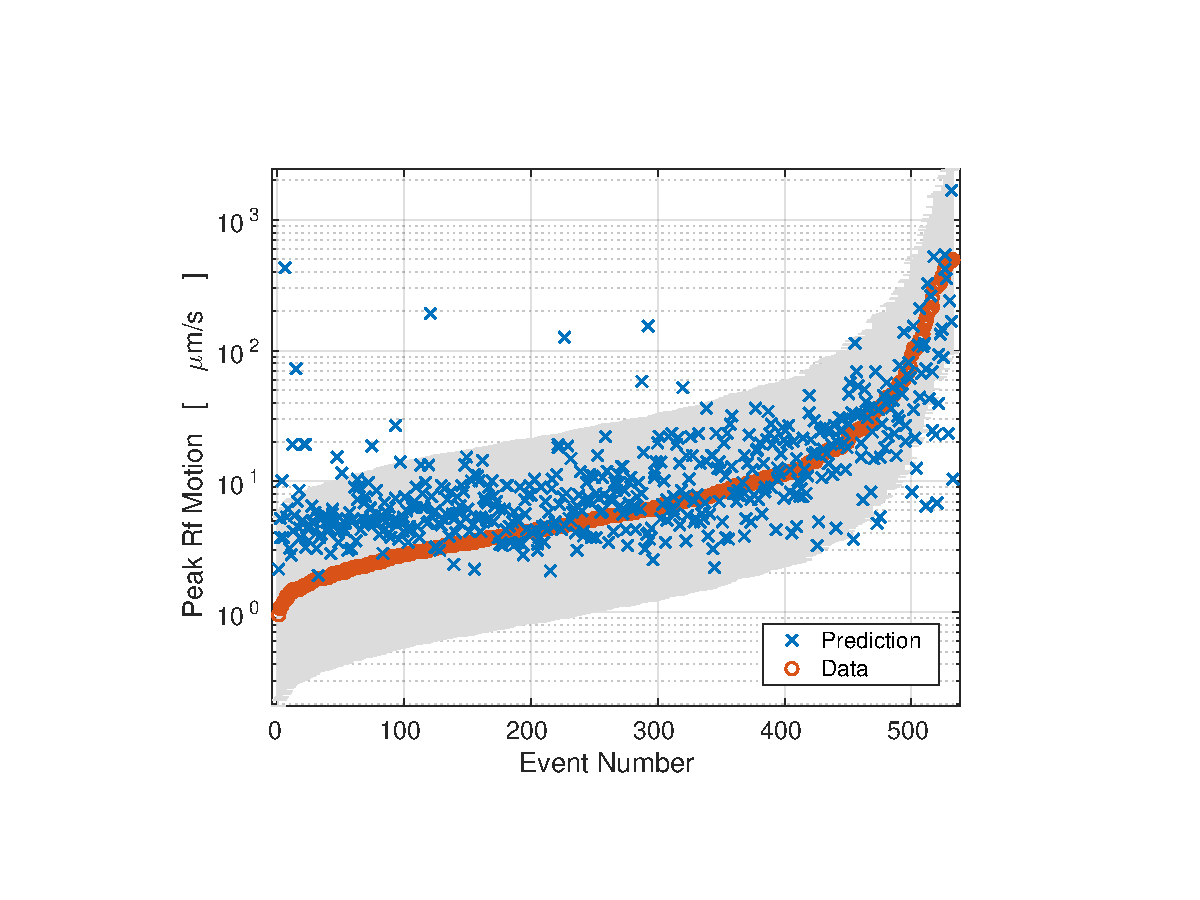
\includegraphics[width=3.5in]{Prediction_LLO_S5_S6.pdf}
 \caption{Fit of peak velocities seen during S5-S6 at the interferometers (LHO and LLO) to equation \ref{eq:Rfamp}.  Fit parameters are estimated from S5-S6 data using final event parameter estimates. The events have been ordered by their measured peak ground velocity (in blue) and the green crosses correspond to the prediction from the equation. About 90\% (LHO and LLO) of events are within a factor of 5 of the predicted value.}
 \label{fig:regression}
\end{figure*}

We now examine the historical earthquake record and predict the likely ground motion seen. We then use seismic data from on-site observations to predict how ground motion will affect the observatories. We have developed an equation attempting to account for physical effects with variable parameters used to fit to the data. Coupling strength of a source at a certain depth to Rayleigh waves, geometric amplitude evolution, and frequency-dependent scaling of the magnitude into ground displacement are taken into account. We estimate the amplitude of the surface waves, $\rm Rf_{amp}$, at the sites using the equation
%Rf_{amp} = 10^{-3} *M*Af*e^{-2*pi*h*fc/cd}*e^{-2*pi*r*fc/ch/Q}/r^{rs}
\begin{equation}
{\rm Rf_{amp}} = M \frac{\rm a}{f_c^{b}} \frac{e^{-2 \pi h f_{\rm c}/c}}{r^{d}}
\label{eq:Rfamp} 
\end{equation}
where $f_{\rm c} = 10^{2.3-M/2}\,\rm Hz$ is the corner frequency of the earthquake,  $M$ is the magnitude of the earthquake, $h$ is the depth, and $c$ is the speed of the surface-waves. Another distance-dependent exponential damping term was included initially, but it did not lead to any improvement in the amplitude prediction. 
%The values of the parameters $a, b, c, d$ are derived from minimizing the difference between the amplitude seen at the interferometer and that predicted by the equation. 
The difference between the prediction ${\rm Rf_{amp}}$ and the set of historical data is then minimized using the parameters $a,b,c,d$.
To do so, we use a Metropolis Hastings Multi-Chain, Monte-Carlo algorithm implementing adaptive simulated annealing, which statistically guarantees obtaining solutions close to global minima \cite{KiGe1983,In2000}. This algorithm was recently used in the optimization of seismometer arrays for gravity gradient noise cancellation in gravitational-wave detectors and a thorough explanation can be found in \cite{CoMu2016}. These are summarized for the gravitational-wave detectors in this study in table~\ref{table:fit} assuming that all physical parameters are in SI units. The regression is shown in figure \ref{fig:regression} for both the LIGO Hanford (LHO) and LIGO Livingston (LLO) gravitational-wave interferometers. For LHO and LLO, the data were taken from November 2005 to October 2007 (Science Run 5 abbreviated as S5) and July 2009 to October 2010 (Science Run 6 abbreviated as S6). We will validate these fits against the latest science run (Observation Run 1 abbreviated as O1)  in the next section. For Virgo, the data were taken from June to September 2011 (Virgo Science Run 4 abbreviated as VSR4). For GEO\,600, the data were taken from July 2010 to June 2011 (GEO High Frequency abbreviated as GEOHF). Figure~\ref{fig:MvsR} shows the peak ground velocity as a function of magnitude and distance for the models. Based on the above equations, we expect that earthquakes with magnitudes greater than 5 can exceed ground velocities of $1\,\mu$m/s.
%$Q = \frac{Q0}{fc^{Qs}}$, 
\begin{table}[]
\centering
\begin{tabular}{|c|c|c|c|c|}
\hline
Detector & $a$ & $b$ & $c$ & $d$ \\ \hline
LHO & 0.16 & 1.31 & 4672.83 & 0.83 \\ \hline
LLO & 0.16 & 1.31 & 4672.83 & 0.81 \\ \hline
VIRGO & 1.60 & 0.89 & 4992.70 & 0.83 \\ \hline
GEO & 8.65 & 1.92 & 324.52 & 1.40 \\ \hline
\end{tabular}
\caption{Best-fit parameters to the peak velocities seen at the interferometers to equation~\ref{eq:Rfamp}.}
\label{table:fit}
\end{table}

\begin{figure}[t]
\hspace*{-0.5cm}
 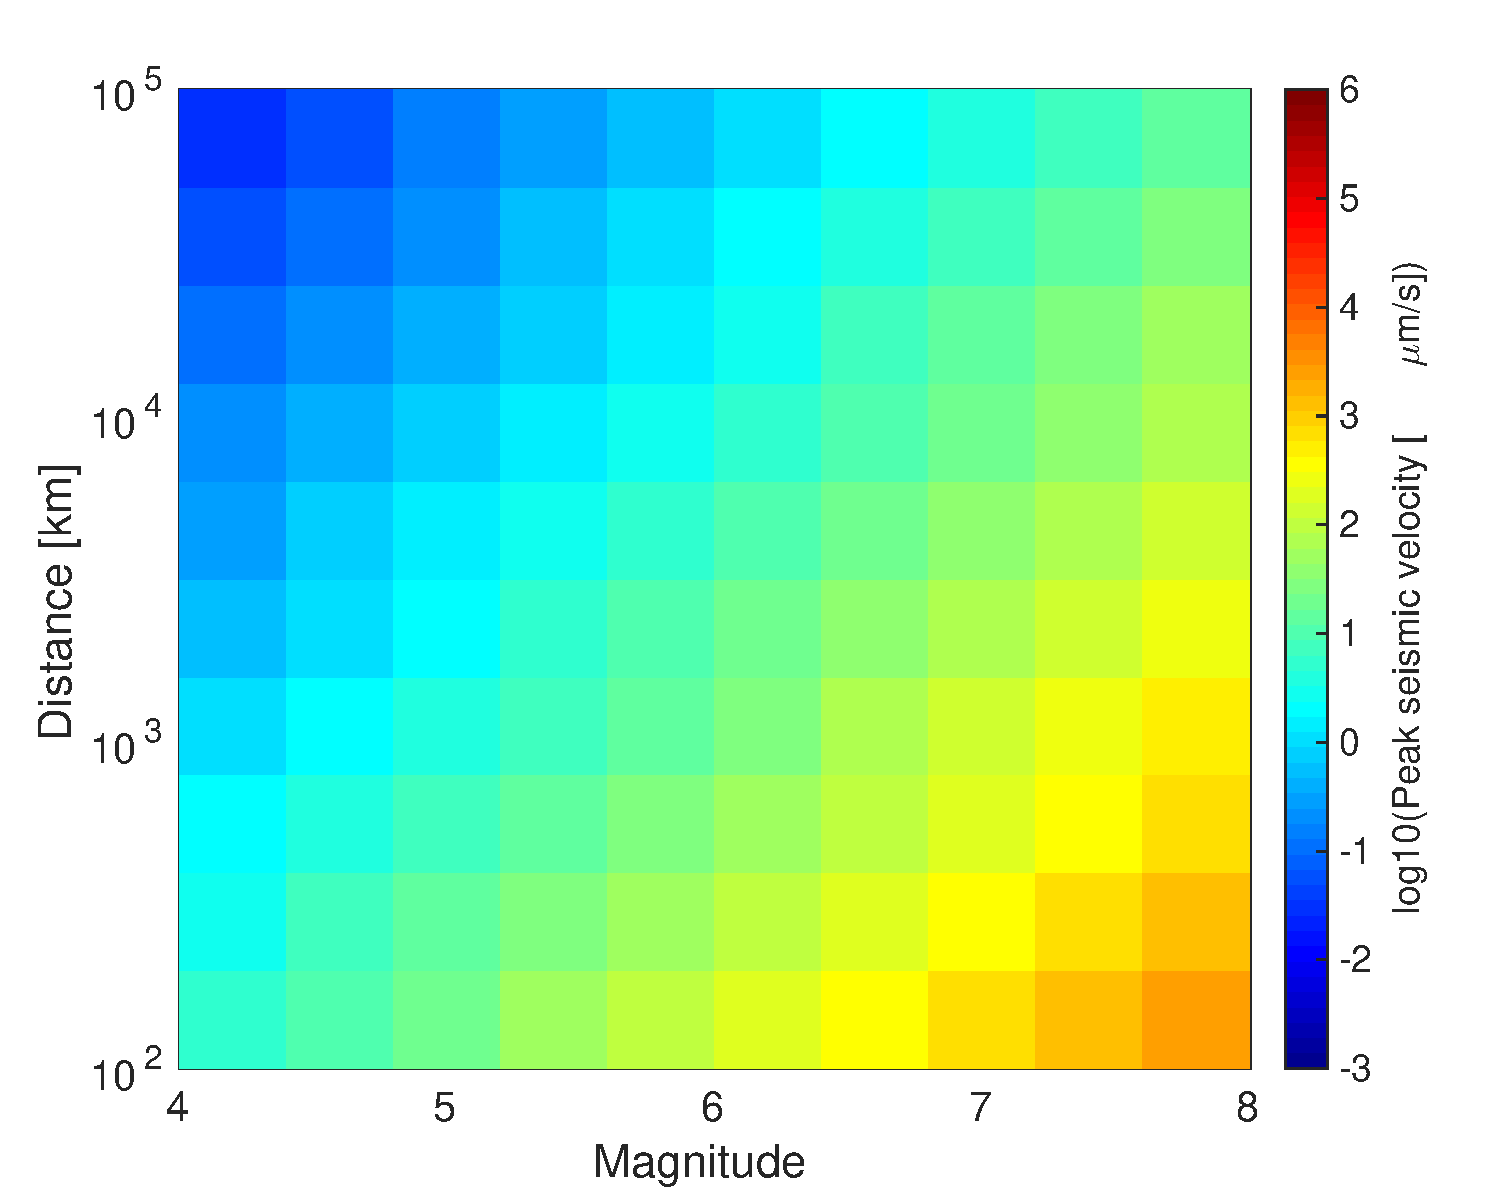
\includegraphics[width=3.5in]{LHO_M_r.pdf}
 \caption{The predicted peak ground velocity as a function of magnitude and distance for LHO (LLO is similar).}
 \label{fig:MvsR}
\end{figure}

\subsection{Site Notification}
The final step of the process is to use the site amplitude and time-of-arrival predictions to create warnings (and possibly detector state changes) for the detectors. The algorithm analyzes the recent notifications and places a threshold on the predictions. We provide a set of site variables that contains the following information. The first is the amplitude prediction for any earthquake expected to be present.
The second is the probability of lockloss, which is discussed in the next section. The third is when this earthquake is expected to arrive at the site.
		
\section{Performance}
\label{sec:performance}

In this section, we provide a number of metrics by which we analyze the performance of \emph{Seismon}.

\subsection{Notification latency}

\begin{figure*}[t]
\hspace*{-0.5cm}
 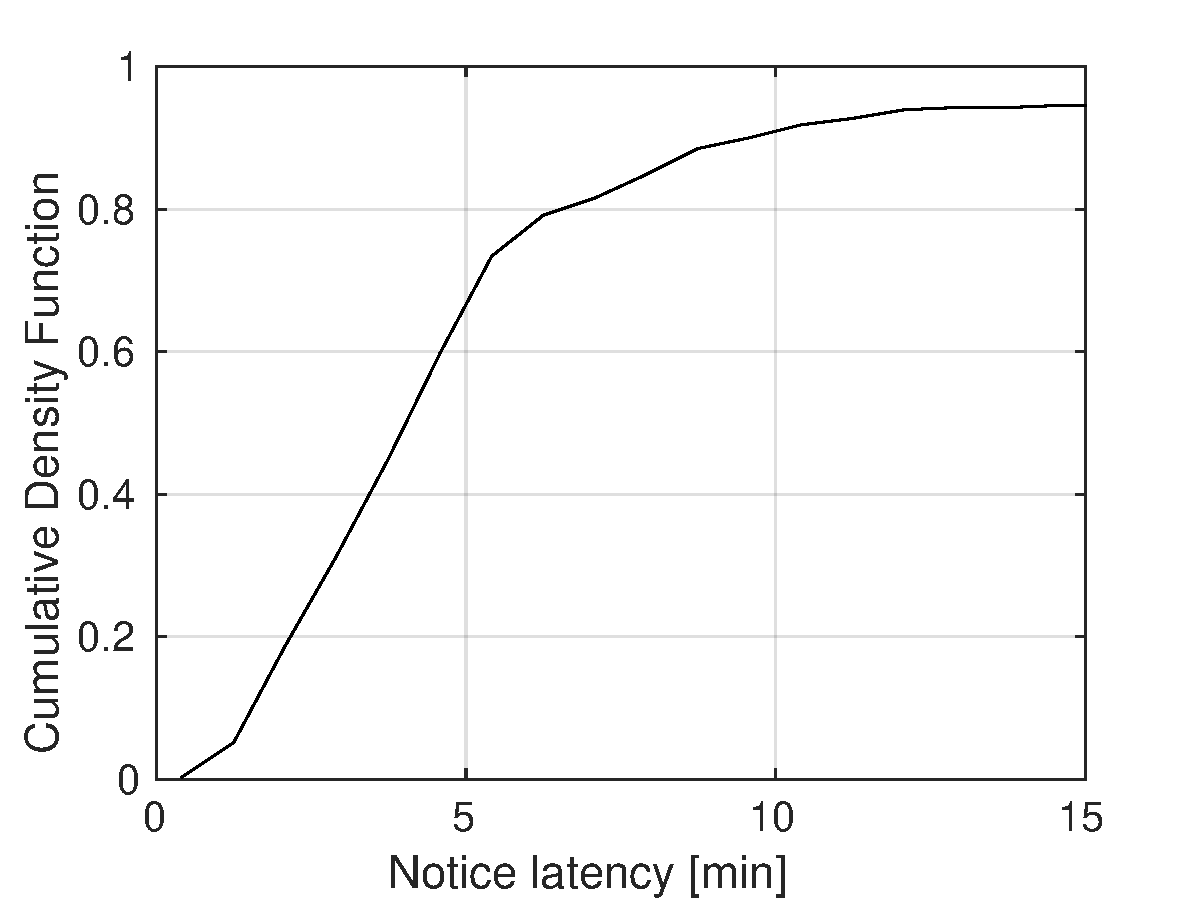
\includegraphics[width=3.5in]{earthquake_notice.pdf}
 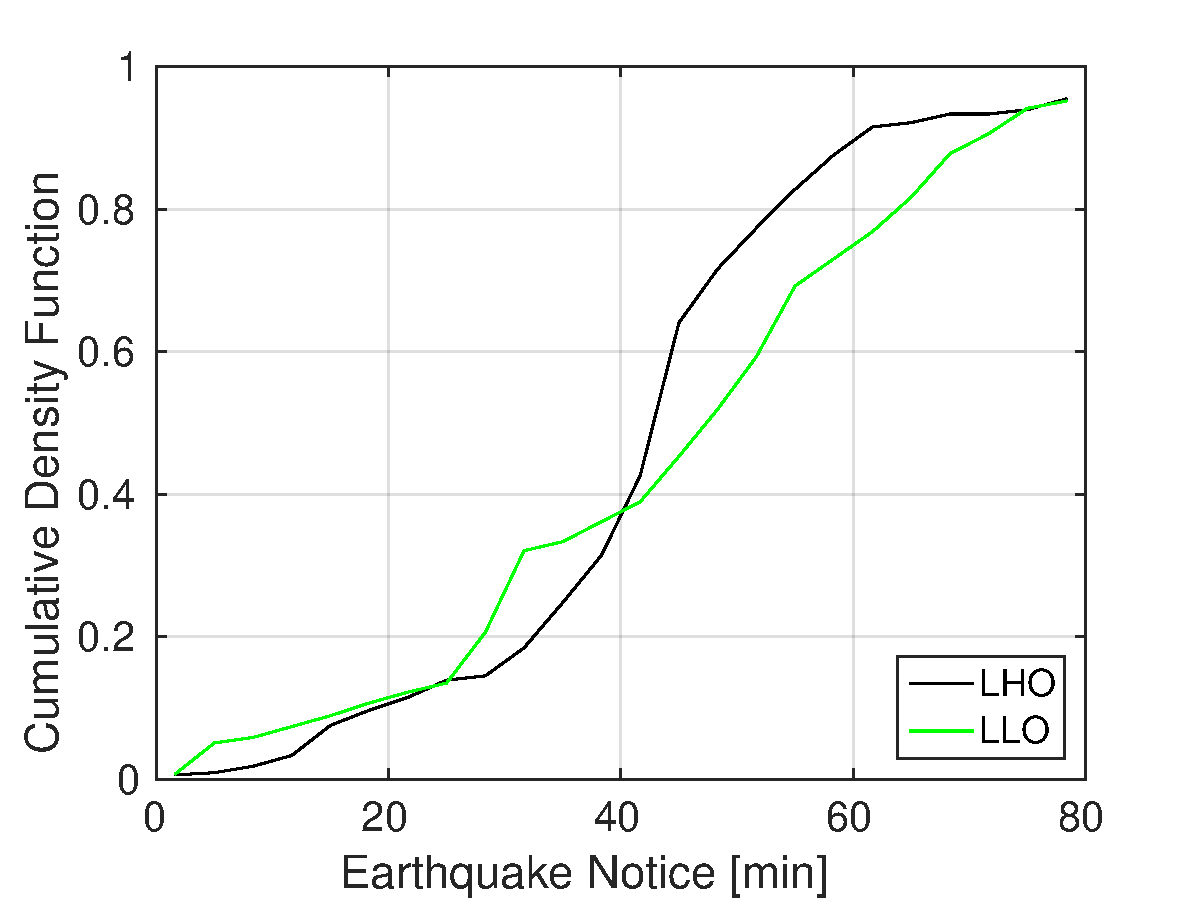
\includegraphics[width=3.5in]{lockloss_notice.pdf}
 \caption{On the left is the time delay between the initiation of fault rupture and generation of the PDL client notification. On the right is the time delay between the earthquake notification from the PDL client and approximate arrival of surface waves at the LIGO Hanford site for global earthquakes. A majority of the locations allow for more than 10 minutes of time between notification and site arrival.}
 \label{fig:delays}
\end{figure*}

One of the most important qualities of an earthquake monitor is the notification latency, or the amount of warning time a detector has to respond to incoming seismic waves. On the left of figure\ref{fig:delays}, we show the time delay between the earthquake and generation of the PDL client notification. In general, notices are generated within 5 minutes of the earthquake. On the right of figure \ref{fig:delays}, we show the cumulative probability distribution of time delays between the notification from the PDL client and approximate arrival of surface waves, assuming surface wave velocities of 3.5\,km/s. In general, there is more than 10 minutes available between notification and surface-wave arrivals. This is more than sufficient time for gravitational-wave detectors to respond by changing control configurations.

\subsection{Ground Velocity Prediction Performance}

\begin{figure}[t]
\hspace*{-0.5cm}
 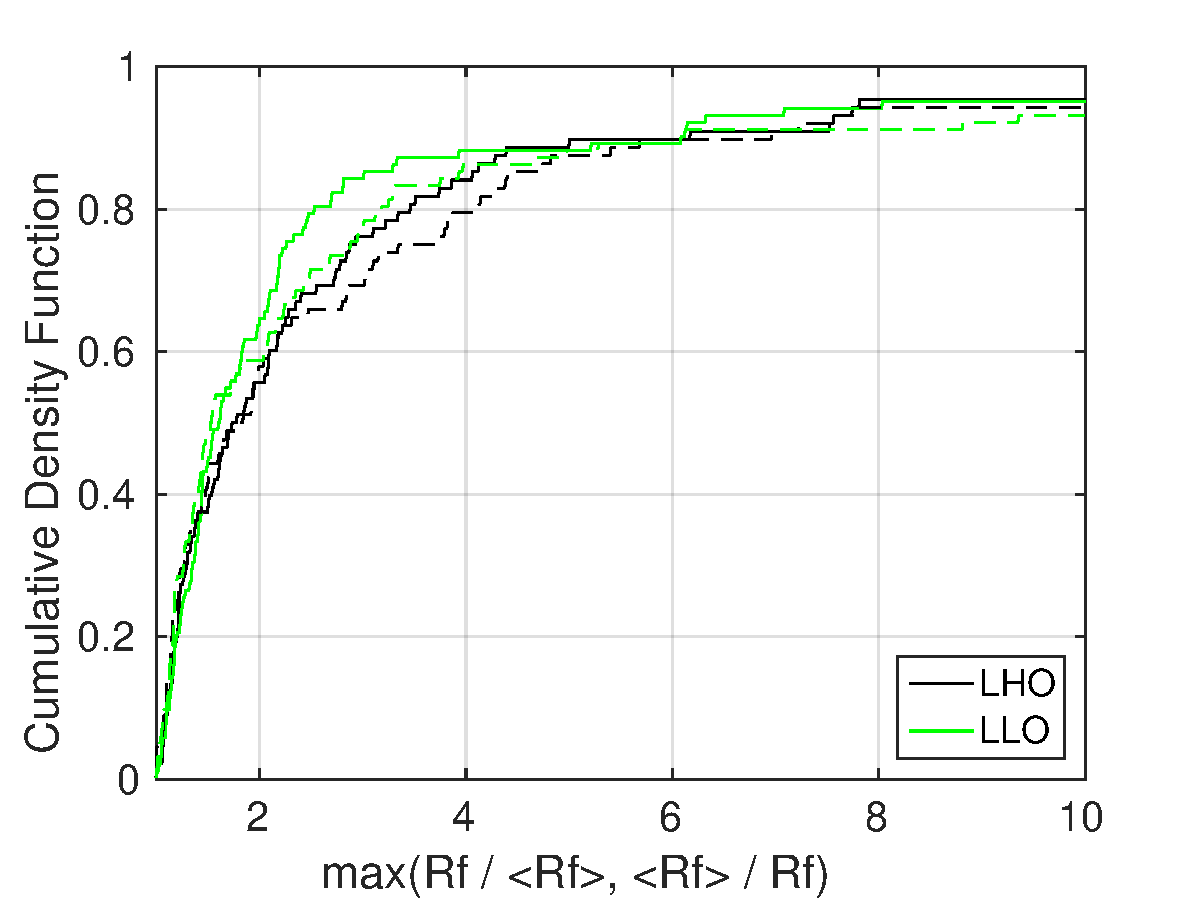
\includegraphics[width=3.5in]{initial_final_vs_real.pdf}
 \caption{Performance of estimation of peak velocities seen during O1 at the interferometers (LHO and LLO) using fit parameters estimated from S5-S6 data. The solid lines use the final earthquake parameter estimates while the dashed lines use the preliminary earthquake estimates. About 90\% of events are within a factor of 5 of the predicted value. The difference in fit parameters due to use of preliminary notices is minimal.}
 \label{fig:regressionperf}
\end{figure}

Another important quality for an earthquake monitor is the accuracy of the ground-motion amplitude prediction and the time-of-arrival.
The ground-motion amplitude performance is evaluated against the most recent science run (Observing Run 1) from September 2015 to January 2016, in figure \ref{fig:regressionperf}. About 90\% of events are within a factor of 5, while those that are not are almost exclusively events that are due to the overlap of many events. This occurs often during aftershocks of large earthquakes. As the largest event is the important one, these are unimportant for predictions. 

As mentioned above, \emph{Seismon} uses the earliest available notices for making time-of-arrival and amplitude predictions. Because the earliest notices may only rely on a few seismometers, as well as the fact that large earthquakes do not fault all at once, the estimates for both magnitude, depth, location, and time can be off. In figure \ref{fig:regressionperf}, we show the difference of arrival times and predicted peak velocities seen during O1 at the interferometers (LHO and LLO) using the initial and final estimates. This is a smaller error than from the regression. 

In figure~\ref{fig:initialvsfinal}, we show the difference between the initial and final estimates of the earthquake time. About 90\% of early estimates are within 3\,s of the final time, which is much smaller than the latency from the generation of the notice itself.
For these reasons, the use of the early notices is not a major source of systematic error for \emph{Seismon}.

\begin{figure}[t]
\hspace*{-0.5cm}
 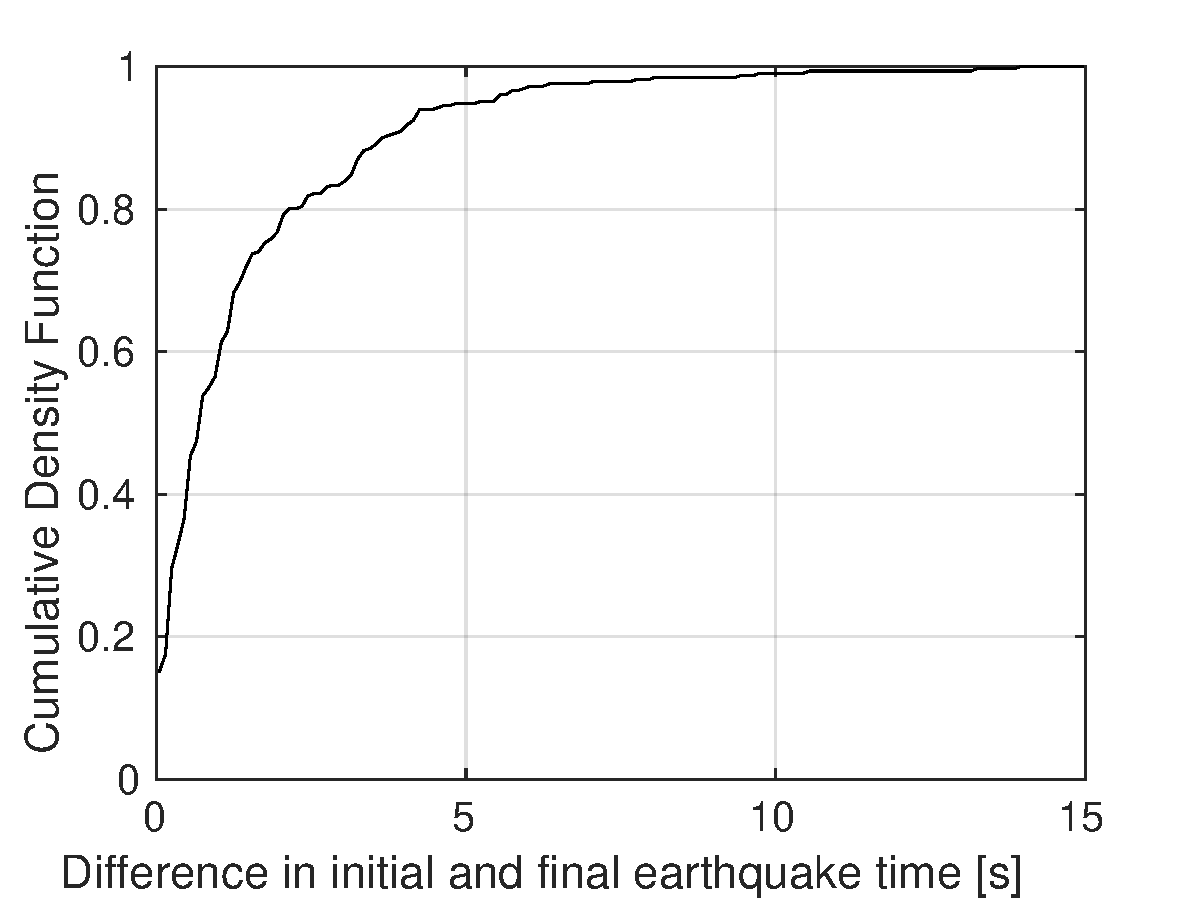
\includegraphics[width=3.5in]{lockloss_est_timediff.pdf}
 \caption{Difference between the initial and final estimates of the earthquake time. About 90\% of early estimates are within 4\,s of the final time.}
 \label{fig:initialvsfinal}
\end{figure}

\subsection{Gravitational-wave detector lockloss prediction performance}

\begin{figure*}[t]
\hspace*{-0.5cm}
 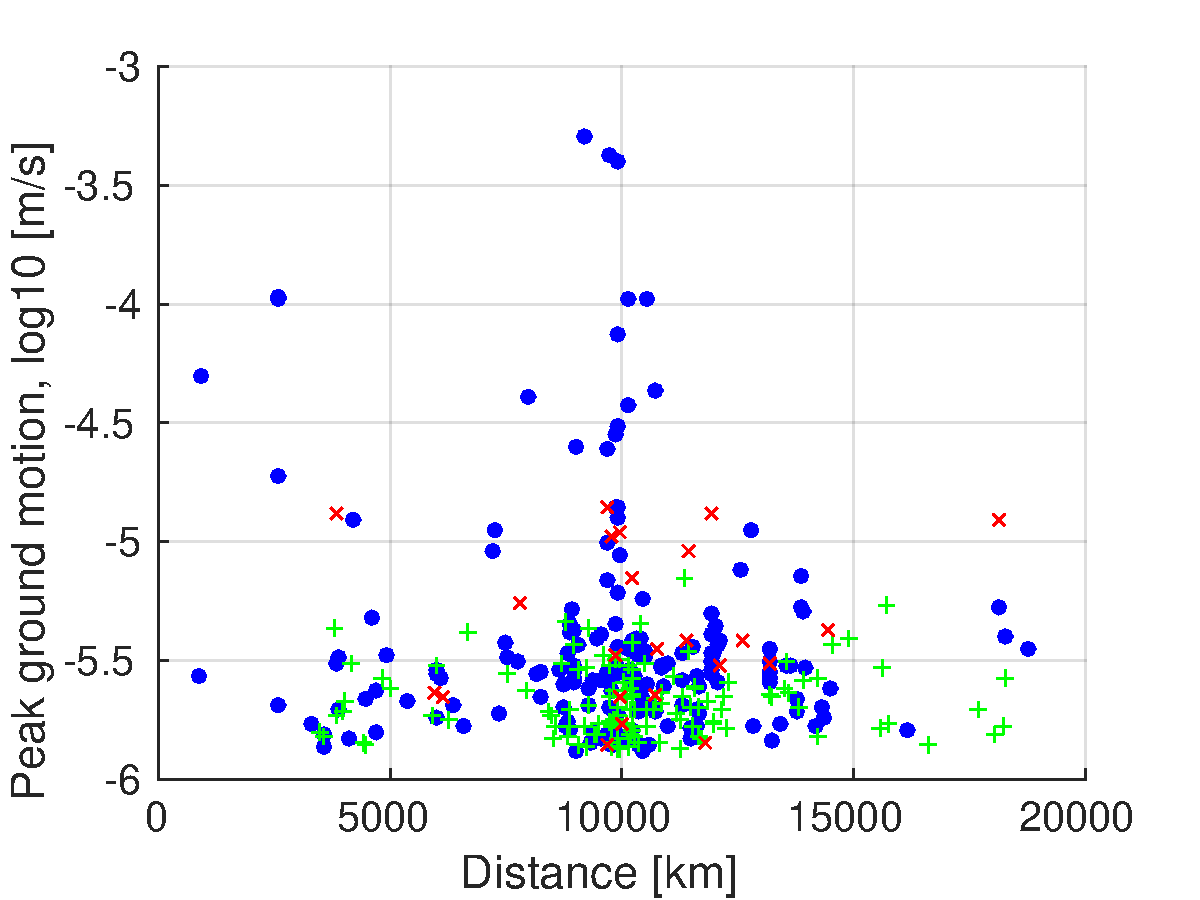
\includegraphics[width=3.5in]{lockloss_vel_distance_LHO.pdf}
  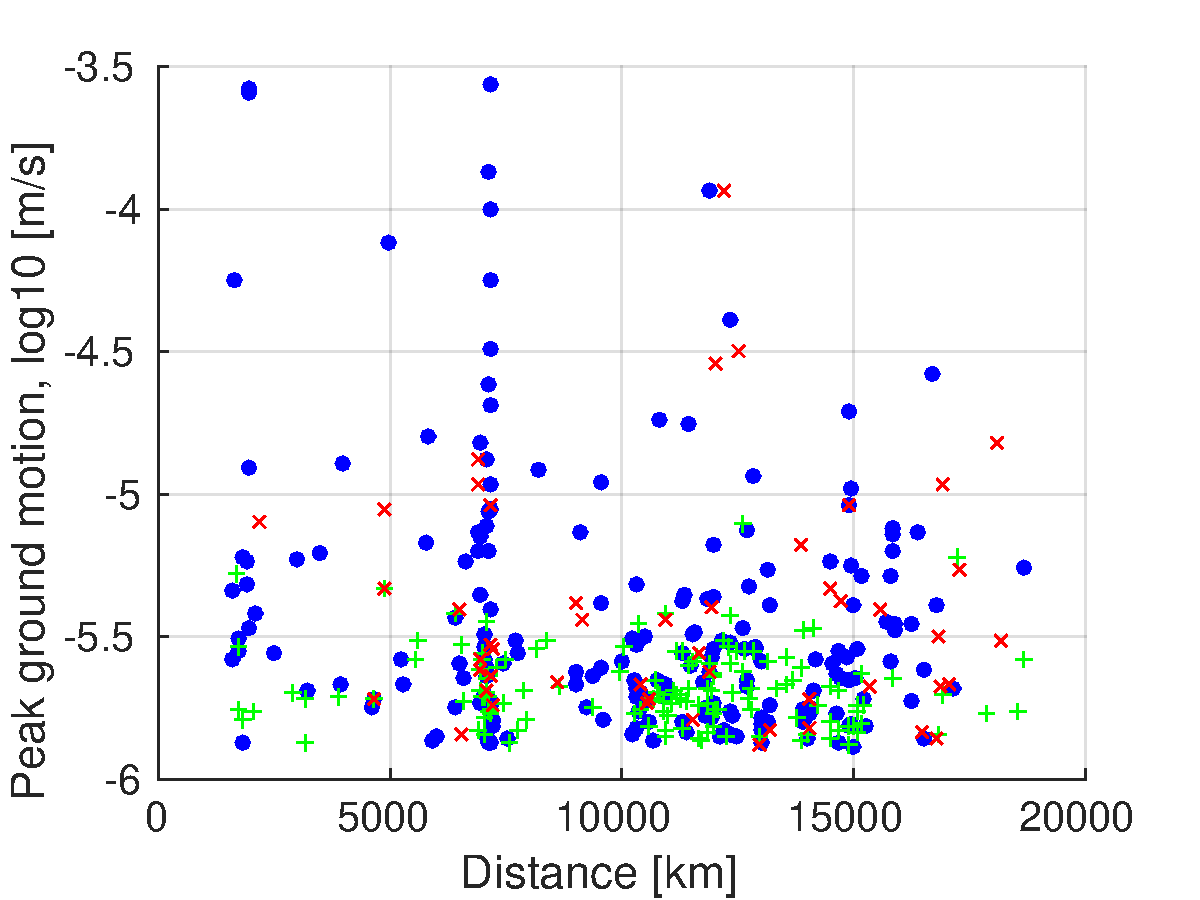
\includegraphics[width=3.5in]{lockloss_vel_distance_LLO.pdf}
 \caption{Lock loss as a function of predicted peak velocity vs. earthquake distance for the gravitational-wave detectors. LHO is on the left and LLO is on the right. Blue circles correspond to times when the detector was not locked, red crosses when the detector lost lock, and green plus signs when the detector stayed locked.}
 \label{fig:lockloss}
\end{figure*}

An earthquake monitor will only be useful for gravitational-wave detectors if it can be determined which earthquakes cause the loss of data (and which will not affect the detector in a significant way).
We now measure the amplitude of the seismic ground motion that causes the detector to lose lock. To do so, we take all known earthquakes above magnitude 5.0 and compute their arrival times. 
We also determine the times that the gravitational-wave detectors fell out of lock during these times. 
We then compare these two figures of merit. 
Fig.~\ref{fig:lockloss} shows these times, both for those times when lock losses occurred, when they did not, and when the detector was not locked. 
The plot shows that while in general ground velocities greater than about 5\,$\mu$m/s lead to lock loss, the situation is complicated at lower ground velocities. This motivates using more than ground velocity to predict lockloss, as for example the spectrum of ground motion or the direction of propagation of seismic waves with respect to the detector orientation.

It is of significant interest to determine the earthquake parameters (and the ground velocities they create) that cause the detectors to lose lock.
Given that \emph{Seismon} is an early warning system, the only parameters available for use are those returned by USGS in low latency, which are magnitude, depth and location (and thus distance). 
In addition, we can use the predicted ground velocity derived from these parameters.
The goal is to predict the outcome of the interferometer lock status based on these parameters.

\begin{figure*}[t]
\hspace*{-0.5cm}
 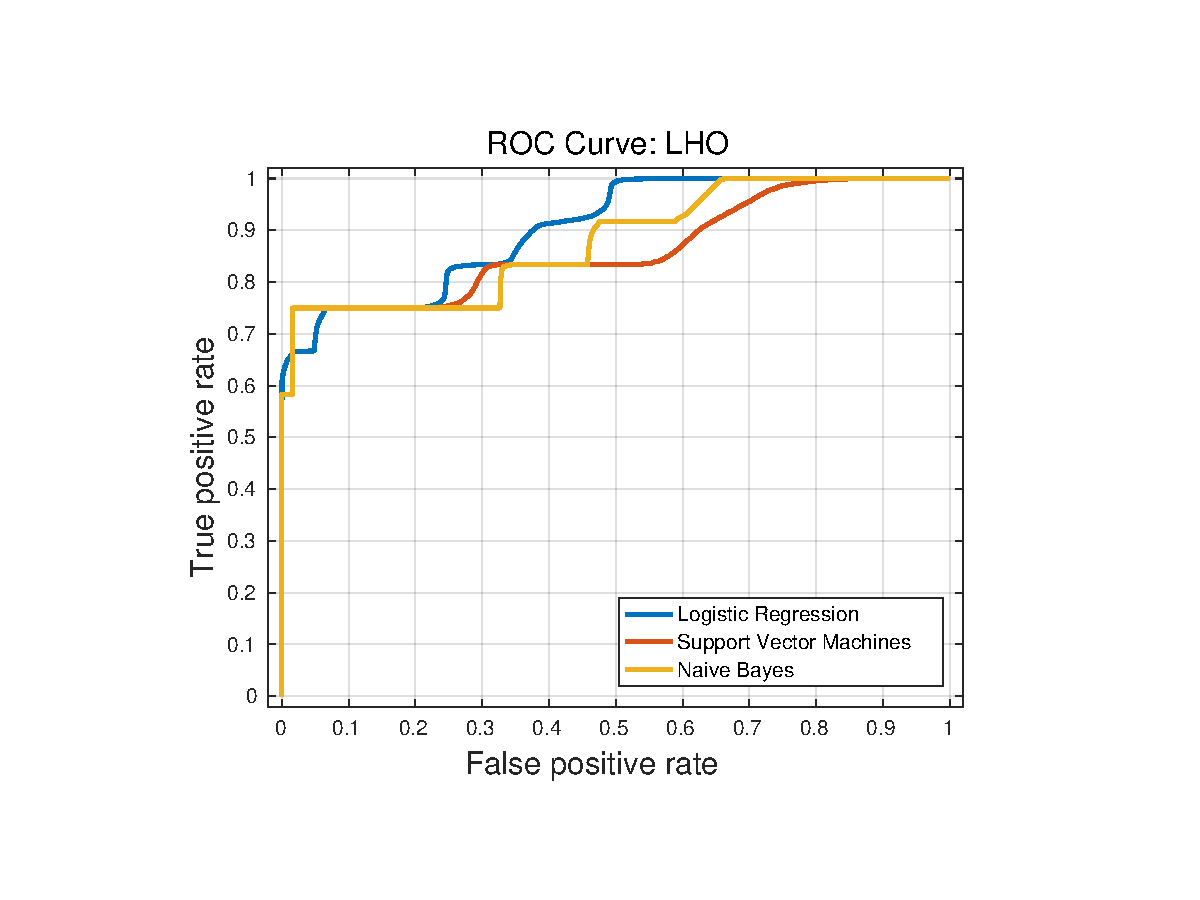
\includegraphics[width=3.5in, trim = 0 4.5cm 0 4.5cm, clip=true]{lho_lockloss_ROC.pdf}
  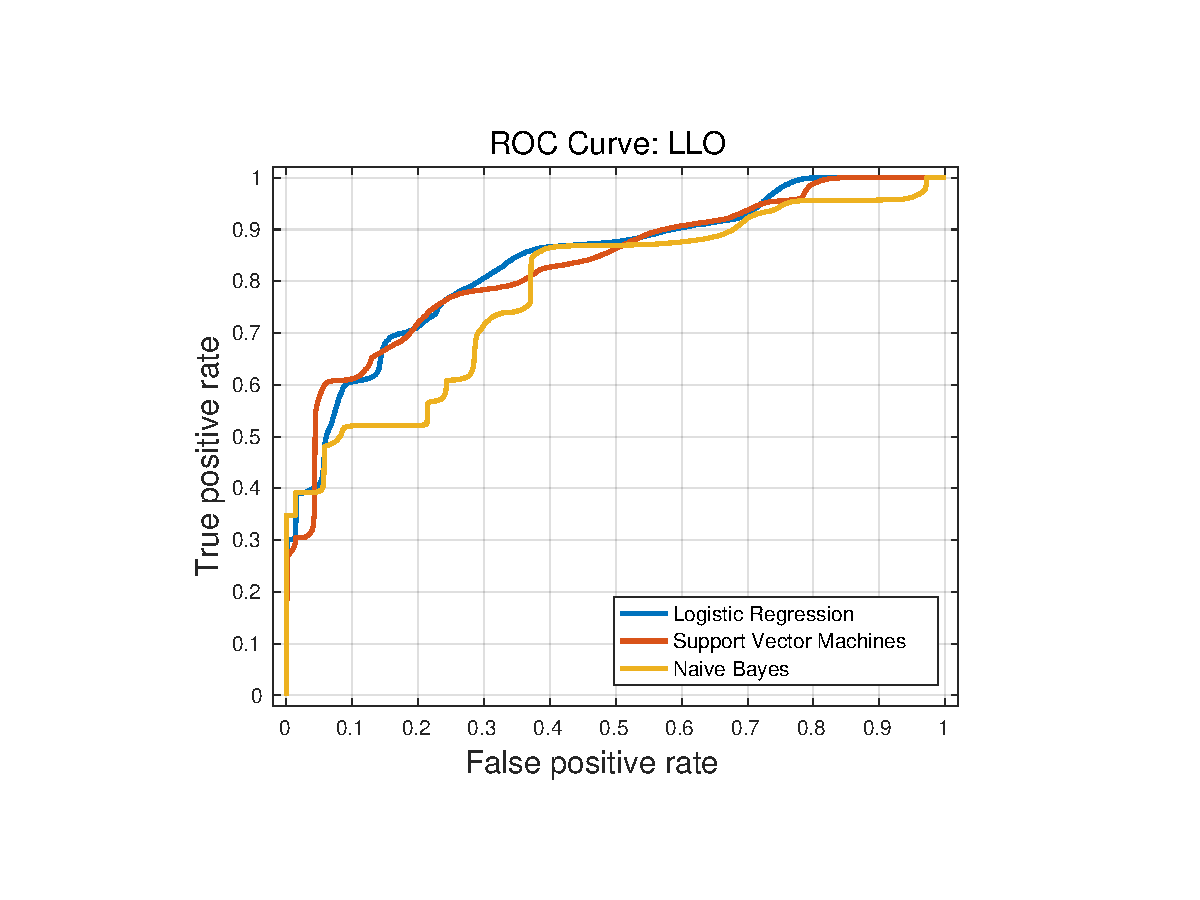
\includegraphics[width=3.5in, trim = 0 4.5cm 0 4.5cm, clip=true]{llo_lockloss_ROC.pdf}
 \caption{Performance comparison of different machine learning classifiers. True positive rate is the ratio of sum of predicted positive condition actually being true to the sum of all actually positive conditions. Positive condition here refers to a lockloss prediction by the classifier which in general can be true or false. False positive rate is the ratio of sum of predicted positive condition being false to the sum of all actually negative conditions. Classifier prediction about the detector being in lock forms the negative condition. A threshold value on classifier output (usually a scaled number between 0 and 1 with value close to unity indicative of lockloss) is varied to generate the receiver operator characteristic curve (ROC).
 }
 \label{fig:MLA_comparison}
\end{figure*}

In the following, we will use a machine learning algorithm to develop a lockloss prediction model. Machine learning algorithms, which are useful for classifying and predicting outcomes for various data analysis problems, have been used in the past with great success in gravitational-wave data analysis \cite{BiBl2013,KyHa2015}. We first compare the performance of different machine learning algorithms aimed at modelling lockloss prediction from the given input parameters.  All three classifiers, Logistic Regression \cite{mccullagh_glm}, Naive Bayes \cite{John_NaiveBayes}, and Support Vector Machine \cite{Burges_SVM}, yield comparable performance with logistic regression giving the best result as is evident from the receiver operator characteristic curve shown in Figure~\ref{fig:MLA_comparison}. 
The classifier with the maximal area under the curve is usually chosen over the others. 

\emph{Seismon} makes lockless predictions using the threshold value obtained from optimal operating point of the ROC curve. 	
The idea is that by setting the false-alarm rate to a certain threshold, we can find an optimum point of efficiency for predicting the outcome. In the analysis that follows, we use $2/3$ of the earthquakes for training and  $1/3$ of the earthquakes for the testing set. 
In general, there is a trade-off between false-alarm probability and efficiency standard probability. The more false alarms one is willing to accept, the higher the rate of earthquakes that will result in lockloss will be caught. For example, if we adopt a false-alarm probability threshold of 0.5, between 90 -- 100\% of earthquakes can be caught.

\section{Conclusion}
\label{sec:conclusions}

In this paper, we have discussed the problem of earthquakes for gravitational-wave detectors and a pipeline designed to minimize their impact. 
We characterize this pipeline in terms of the warning time for these experiments.
We have shown that the earthquake warning system can both predict likely earthquake arrival times and ground velocity amplitudes. 

A code that performs these steps is available at https://github.com/ligovirgo/seismon/ for public download. Hopefully, this will allow other researchers to easily use the fits. Required inputs are the latitude and longitude of the site and magnitude, latitude, longitude and depth of the source.

In the future, this algorithm will be applied to the next science run. It will require coordination between the low-latency notification software and the detector control systems to maximize the utility of the system. 
Further effort needs to be spent on investigating the effect of strong ground motion on the detector control system.
This will include studies of the control configuration best for riding out times of large ground motion.

\section{Acknowledgments}
MC was supported by the National Science Foundation Graduate Research Fellowship
Program, under NSF grant number DGE 1144152. 
NM acknowledges Council for Scientific and Industrial Research (CSIR), India for providing financial support as Senior Research Fellow.  
LIGO was constructed by the California Institute of Technology and Massachusetts Institute of Technology with funding from the National Science Foundation and operates under cooperative agreement PHY-0757058.
This paper has been assigned LIGO document number LIGO-P1600321.
The authors would like to thank Dr. Jenne Driggers for a detailed reading of an early version of the manuscript.

%\raggedright
\bibliographystyle{unsrt}
\bibliography{references}


\end{document} 
